\documentclass[12pt,a4paper,titlepage,oneside,openany]{article}

\title{Critical Path Method}
\date{\today}
\author{
	Management von Softwareprojekten (Gruppe 4):\\
	Florian St\"auble \email{e0415588@student.tuwien.ac.at},\\
	Clemens Sauerwein \email{e0716649@student.tuwien.ac.at},\\
	Thomas Chrenko \email{thomas@chrenko.at},\\
	Silvio Riener \email{silvio@riener.ws} and\\
	Mathias Ertl \email{e0326788@student.tuwien.ac.at}
	}
\setlength{\parskip}{5pt plus 2pt minus 1pt}  % Abstand zwischen Absaetzen
\sloppy

% apperantly set the font to arial:
\renewcommand{\rmdefault}{phv} % Arial
\renewcommand{\sfdefault}{phv} % Arial

% page format:
\usepackage{geometry}
\geometry{a4paper,top=25mm,left=25mm,right=25mm,bottom=25mm,headsep=10mm,footskip=12mm}
%\parindent0pt


% various packages:
\usepackage{hyperref}
\usepackage{graphicx}


\usepackage{cite}

% encoding:
%\usepackage{ucs}
%\usepackage[utf8x]{inputenc}
%\usepackage[OT1,T1]{fontenc}
%\usepackage{ae,aecompl}

% new comand:
\newcommand{\email}[1]{\href{mailto:#1}{$<$#1$>$}}
\newcommand{\cpm}{\emph{Critical Path Method}}

\begin{document}
\maketitle
\begin{abstract}
This seminar paper deals extensively with the critical path method developed by
Morgan R. Walker and James E. Kelly in the late 1950s\cite{Kelley:1959:CPS:1460299.1460318}.
Despite the age of this
method, it is still widely used in a lot of different projects.  This paper is
divided into five chapters, each dealing with an important part of the critical
path method. 

Chapter one provides a short introduction into the topic, some background
information about the critical path method and definitions of some very
important catchwords. Furthermore the history of the critical path method is
outlined. 

In the subsequent chapter, the critical path method itself is described very
detailed, it is explained how information gained with the critical path method
can be interpreted and how to react on this information in a proper way (if
necessary).

Chapter three deals with different algorithms used to determine the critical
path of a project.  The mentioned algorithms appear in different tools, which
are used to determine the critical path of a project. 

In the fourth chapter, advantages and disadvantages of the critical path method
are outlined. Furthermore possible alternatives and advancements are mentioned
and described. 

Last but not least chapter five explains how the critical path method is used in
everyday project management, which project management tools support the critical
path method and a short introduction to this tools.

The conclusion is a short recap of all important findings made throughout this
seminar paper.

\end{abstract}
\tableofcontents

\section{Introduction}
% Background, Scope (5 Seiten) - Silvio

This first chapter provides a short introduction into the critical path method and some noteworthy
background information.

First of all it should be mentioned, that there exist a lot (100+) different names for  the critical
path method like “network scheduling”, “critical path analysis” or “critical path method”. According
to \cite{dua} there is no basic difference between this differently named methods. For the readers
convenience, in this seminar paper the method is always called critical path method (CPM). 

The critical path method is a widely used project management tool, which allows the scheduling of
activities in a project. It is not only used in software development but even in construction
projects, production projects, research projects, and a lot more. The critical path method can be
used for every project, consisting of different, interdependent activities.  

The purpose of the critical path method is to calculate\cite{santiago}:
\begin{itemize}
  \item The longest path of planned activities to the end of the project.
  \item The earliest and latest that each activity can start and finish without making the project longer.
\end{itemize}

A quote from an unknown reviewer of the book \cite{obrien} describes the critical path
method very well:

\begin{quotation}
Perhaps the most ironic aspect of the critical path method is that after you understand it, it is
self-evident. Just as an algebra student can apply the rules without full appreciation of the power
of the mathematical concepts, so can the individual apply CPM or its equivalent without fully
appreciating the applicability of the method.
\end{quotation}

Activities on this critical path should be monitored very closely, and it is important to make sure
that such activities are completed in time. 

The critical path method is divided into 3 phases:
\begin{description}
  \item[Phase 1] Break project into activities.
  \item[Phase 2] Create time estimates for each activity. 
  \item[Phase 3] Create a time-cost relationship.
\end{description}

Each phase is described in more detail in chapter 2.

Generally it can be said, that the CPM is a very powerful method to receive important information
about a project. It shows which activities in a project are most important, which activities can be
carried out in parallel, how much resources are needed, when the project can be finished, when it
will be finished according to the current state and it is possible to get an overview of all
activities which have to be carried out.

\subsection{CPM – what for?}

Basically CPM is part of a scheduling technique as everyone uses it every day – just a bit more
advanced. For a single person scheduling of it’s everyday activities is rather easy (taking a
shower, dressing up, …), but can get quite challenging if the person is stressed or if more task
should be done at the same time. If it is necessary to schedule the tasks of two persons this is
even more challenging, for three or more persons it is nearly impossible without a well-defined,
structured method. Mapping all this to an industry project, a lot of different tasks have to be
managed, and each task must be finished at a specific time. CPM allows saving time through better
planning and as everywhere in industry time is money.

In December 1957 an experiment was started, to show the efficiency of the critical path method. Two
teams consisting of different engineers were set up, one team had to use an early version of CPM (at
this time called Kelly-Walker method) the other team used traditional planning methods. Both groups
had to plan a ten million \$ chemical plant in Louisville, Kentucky. Of course both team worked
completely independent of each other. The members of the CPM group received and introduction course
(40h) to CPM. All in all, the project contained a network of more then 800 activities. After six
month, major changes (about 40\% of the whole project) had to be taken into account. For the CPM team
the modification and recomputation of the plan took only about 10\% of the original planning time –
much better then the normal scheduling group.  Another major advantage of the CPM team was the
ability to identify critical delivery items. The CPM team identified this critical delivery items
from the analysis of their network plan, while the normal scheduling group selected randomly
critical delivery items\cite{obrien}. 

This example shows that by using CPM a lot of time and effort can be spared. 

\subsection{History of the CPM}

Research in the field of project management and activity scheduling was done because of the need of
a method to plan and control complicated projects. 

As previously mentioned the critical path method was invented in the year 1959 by Morgan R. Walker
(DuPont) and James E. Kelly (Remington Rand).  Some other organizations claim that they invented the
critical path method (UK Central Electricity Generating Board and the US Navy) but officially the
chemical company DuPont invented it. The critical path method was based on a graphic network
commonly known as the “arrow method”.  The advantages of the critical path method were discovered by
many organizations especially construction companies who quickly integrated the CPM in their daily
project management. 

Not only in the private sector, but even in the military sector such a method was required.
Therefore the US Navy started the project “Program Evaluation Research Task” codename PERT. Its goal
was to develop a way to “plan and control complicated projects”. According to the phase II report of
the PERT program, the method needs to provide following possibilities.

\begin{enumerate}
  \item Increased orderliness and consistency in planning and evaluating.
  \item An automatic mechanism for identifying potential trouble spots.
  \item Operational flexibility for a program by allowing for a simulation    of schedules.
  \item Rapid handling and analysis of integrated data to permit expeditious corrections.
\end{enumerate}

An outcome of this project was the first arrow diagram (developed by Dr. C.E. Clark). The PERT
project was later renamed in “Program Evaluation and Review Technique” and used in multiple large
scale projects like the “Fleet Ballistic Missle Program” with over 3000 parties involved. It is
said, that Morgen Walker and James Kelly took some ideas and the term “critical path” from this PERT
project\cite[p. 10]{obrien}.

In the year 1961 an advanced version of the CPM was presented by Professor Fondahl of the Stanford
University – this version was called “precedence method”. The precedence method was an improvement
in respect of schedule construction and analysis. Additionally, after this update by Prof. Fondahl,
the critical path method even was able to assist in the organization of resources. This is the
method, which is currently used in most projects\cite{Uher}.

The probably best known project which made use of the critical path method is the Apollo 11 mission
of the NASA. During this mission two persons were landed on the moon (Neil Armstrong, Buzz Aldrin)
on July 20, 1969. About two million tasks led to the moon landing. 

\subsection{Important terms}

In this part some important terms are introduced and described as detailed as needed for this
seminar paper. 

\begin{description}
  \item[Float (slack):] Is the amount of time an activity can be delayed without affecting succeeding tasks
(free float) or the completion date of the project (total float). When using CPM in software
development, the float is mostly called buffer. 
  \item[Critical activity:] Is an activity with zero buffer, therefore an activity on the critical path. 
  \item[Critical path:] The critical path is a series of activities, whose duration is the minimal amount of
time needed to complete the project.  If an activity on the critical path is delayed, the whole
project is affected and delayed. A project can have several, parallel critical paths.
  \item[Early finish date (EF):] The EF is the earliest possible point in time on which the project (or an
activity) can be finished. The EF needs to be changed, if activities on the critical path are
delayed. 
  \item[Early start date (ES):] The ES is the earliest possible point in time on which the project (or an
activity) can start. 
  \item[Late finish date (LF):] The LF is the latest possible point in time on which the project (or an
activity) must be finished, in order not to delay a specific milestone or a fixed handover date.
  \item[Latest start date (LS):] The LS is the latest possible point in time on which the project (or an
activity) must start (based on previous effort estimation) in order not to delay a specific
milestone or a fixed handover date.
\end{description}

\subsection{Summary}
Chapter one provides a short introduction into the critical path method. First of all it is
outlined, that the critical path method is a project management tool, which can be used in nearly
every kind of project, which consists of interdependent activities. Afterwards it is described which
information about the project can be obtained with the help of the critical path method and how to
handle this information.  

After the introduction an experiment of the year 1959 is presented. This experiments shows the
advantages of the critical path method compared to traditional methods. 

The third part of chapter one is a look into the past of the critical path method. It is explained
that Morgan Walker and James Kelly developed this method; it is even mentioned why they created this
method and which other approaches exist.  

The last part of chapter one is an introduction of important terms in respect of the critical path
method. The two most important terms are float (how much a task can be delayed) and of course
critical path (shortest path to the end of the project)\cite{santiago}.

\section{The Critical Path Method}
Eigentliche Beschreibung der Methode (5 Seiten) - Mathias

\section{Manual Compution and Technical Information}

This chapter first provides the necessary formulas for calculating CPM-diagrams and then the manual computation of the most important values of a CPM-diagram are explained by a specific example. In the course of this manual computation it is also shown how the Critical-Path itself can easily be determined by hand.

\subsection{Formulas} \label{formulas}

This section uses the terms explained in chapter REFERENCE-To-The-Important-Terms-Stuff and shows how these definitions depend on each other.
First the forward- and backward-pass, two important concepts in calculating times are explained, then the TF (total Float) is expressed by the definitions already known.
\subsubsection{Forward Pass} \label{forwardPass}
The "forward pass" deals with the Question "how early can a project be completed?". To answer this question Start and End-Times for each activity have to be calculated, specifically as states in the Terms definition the ES (early start) and EF (early finish).

The first activity of a new Project must have a date manually set, but by definition and for the purpose of these calculations it is assumed that the first activity starts at time 0. Therefore the ES of this first start activity is also 0.
\begin{equation}
ES_{0} = 0
\end{equation}

The EF is simply the the duration added to the ES-Date:
\begin{equation}
EF = ES + D
\end{equation}

For the formula to calculate the ES of an activity the Definition of Latest Early Finish (LEF) is needed. In the event that there is more then 1 predecessor activity the LEF is the latest EF of any of these predecessors.

With this information ES can now be defined as follows:
\begin{equation}
ES = LEF_{PRED}
\end{equation}

\subsubsection{Backward Pass}
The backward pass deals with the question "How late can an activity start without delaying the project".
For this question to answer the LS (Late Start) and LF (Late Finish) must be calculated.
By definition the latest finish time (LF) of the last activity or event is traditionally equal to the earliest finish time (EF). This is because it is assumed that it's economic to complete a project in as less time as possible. This might not be always the case, depending on cost factors etc., but for the CPM algorithm it is expressed as follows:
\begin{equation}
LF_{last} = EF_{last}
\end{equation}
 
Newer version of the CPM algorithm allow the user to set a FNET (finish not later than) Date for activities, but the original algorithm didn't have this option.
 
 
The LS is fined as:
\begin{equation}
LS = LF - D
\end{equation}
 
Working backward from an activity shows that the LF depends on the successor activity and is defined as follows:
\begin{equation}
LF = ELS_{SUCC}
\end{equation}
In this context ELS (Earliest late start) is the earliest LS of any successor activity.

A \emph{second} backward pass enables us to calculate more interesting attributes. The \emph{free
float} ($FF$) is the difference between the earliest start of any succeeding activity and the early
finish of the respective activity. It thus represents the amount of time by which an activity can be
delayed without delaying the entire project.  The \emph{independent float} ($IF$) is defined as the
difference between the earliest early start of any succeeding activity and the latest early finish 
of any proceeding activities. The formulas are given in (\ref{eq:backward_pass_two}).

\begin{eqnarray}
&& FF=EES_{succ}-EF \nonumber\\
&& IF=EES_{succ}-LEF{pred}-D \\
\label{eq:backward_pass_two}
\end{eqnarray}
 
\subsubsection{Total Float}
 
 When knowing either LS and ES  or LF and EF the total Float (TF) for an activity can be calculated by the formulas:
\begin{equation}
	TF = LS - ES
\end{equation}	

\begin{equation}
TF = LF - EF
\end{equation} 




\subsection{Determining the Critical Path} \label{determine_crit_path}
The information compiled in the previous sections is now ready to be used to find the \emph{critical
paths} of the project. This is of course the quintessential part of the \cpm{} that gives it a
decisive advantage over a much simpler bar chart or an even simpler todo-list.

A critical activity is, as described in the Important terms - section, a activity which must not get delayed for the project to finish as early as possible and therefore lies on the critical path. Since there may be more than one critical path in a project, the following three conditions must hold that a single activity is a critical activity:

\begin{enumerate}
	\item The early and late start times at the activity completion must be equal. $ ES = LS $
	\item The early and late finish times at the activity completion must be equal. $ EF = LF $
	\item The difference between the ES and LF must equal the duration. $ |ES - LF| = D $
\end{enumerate}

The first 2 Conditions are very easily seen after calculating ES, EF, LS, LF for each activity. The third condition is a bit more tricky, since an extra calculation has to be made for each activity.
Furthermore, each critical activity must follow at least one other critical activity(unless of course it is the last activity), meaning that a critical-path cannot be interrupted. It is however possible for a critical path to spread out into a number of paths, and these paths can converge again into one.



\subsection{Manual Calculation of CPM-Method by Example}
In this section the manual calculation of the CPM-method is shown via the following example project plan:
\begin{figure}[h] 
\centerline{\fbox{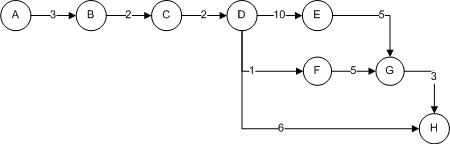
\includegraphics[width=130mm]{img/computation1.png}}}
\caption{Project Plan}
\label{pic:plan1}
\end{figure}
While usually the nodes are labeled with numbers, in this example the nodes are labeled with letters and the numbers are the duration of the activity. For example the activity AB has the duration 3.

\subsubsection{Forward Pass and Early Event Time}
As described at \ref{forwardPass} first the forward Pass is made determining the earliest finish time of the project and ES and EF of activities.

The project starts at event A, and therefore event A is labelled with 0. (Figure ~\ref{pic:plan2})
\begin{figure}[h] 
\centerline{\fbox{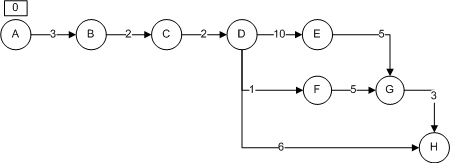
\includegraphics[width=130mm]{img/computation2.png}}}
\label{pic:plan2}
\caption{Project Plan}
\end{figure}
After this it is easy to determine that event B can be reached within 3t, since there is only activity AB in between with duration 3t. Event B is therefore labelled with 3.
To reach event C two activities namely AB and BC are necessary, which durations 3 and 2, therefore the earliest time even C can be reached is $3+2 = 5$. Event C is labelled with 5. (Figure ~\ref{pic:plan3})
\begin{figure}[h] 
\centerline{\fbox{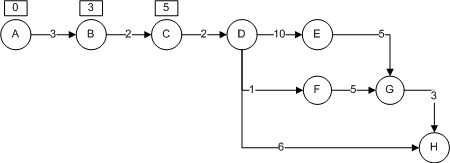
\includegraphics[width=130mm]{img/computation3.png}}}
\label{pic:plan3}
\caption{Project Plan - Step 2}
\end{figure}

Calculating the same for events D, E and F the diagram looks as shown in figure ~\ref{fig:plan4}.
\begin{figure}[h] 
\centerline{\fbox{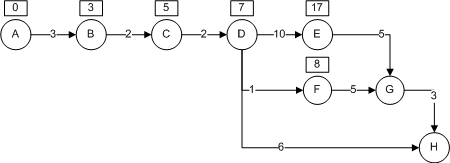
\includegraphics[width=130mm]{img/computation4.png}}}
\label{fig:plan4}
\caption{}
\end{figure}

Event G has to activities that lead into it, EG and FG, which both have the duration 5, but different time-labels (17 and 8). The label of event G is calculated by $ max(label E + duration EG, label F + duration FG) = max(17+5, 8+5) = max(22,13) = 22 $. Doing the same for event H the diagrams looks like figure ~\ref{pic:plan5}.
\begin{figure}[h] 
\centerline{\fbox{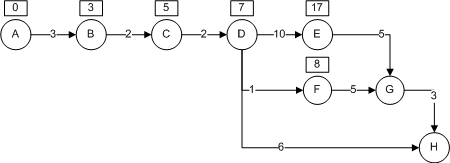
\includegraphics[width=130mm]{img/computation4.png}}}
\label{pic:plan5}
\caption{Project Plan - Step 3}
\end{figure}
\subsubsection{Backwards Pass and Late Event Time}
 Secondly the backward pass is done to determine the Late Event Time and subsequently the LS and LF for each activity.
 The backward pass is basically the same as the forward pass, with the different that the last node is the starting node and the network is worked from the last node to the first node.

In this example the start-node for the backwards pass is event H with late event time 25. Event G for example is labeled with $ 25-3 = 22 $, and when 2 different activities lead into one event is is labelled the maximum of the predecessor-event (predecessor in the backward sense) minus the duration of the activity. This leads to the following diagram:
\begin{figure}[h] 
\centerline{\fbox{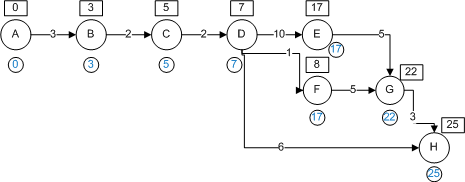
\includegraphics[width=130mm]{img/computation6.png}}}
\label{pic:plan6}
\caption{final project plan}
\end{figure}
The values added with the backward pass are in blue underneath each event.

\subsubsection{Activity Start and Finish Times}
From figure ~\ref{pic:plan6} we can determine the ES, EF, LS, LF and TF of each activity. A typical activity looks as follows:
\begin{figure}[h] 
\centerline{\fbox{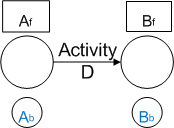
\includegraphics{img/activity_plan.png}}}
\label{pic:activity_plan}
\caption{activity legend}
\end{figure}
Each activity is bound by 2 events and has a Duration (D) and after completing the forward the ES can be calculated as follows:
\begin{equation}
ES = A_{f}
\end{equation}
If ES of an activity is know the EF can easily be determined by ES and B.
\begin{equation}
EF = ES + D
\end{equation}

If the backward pass was also completed successfully LF can be expressed as
\begin{equation}
LF = B_{b}
\end{equation}

After LF, the LS is obviously
\begin{equation}
LS = LF - D
\end{equation}

\subsubsection{Critical Path}

When applying the rules of \ref{determine_crit_path} the each activity is easily marked as critical or non-critical and the critical path becomes visible:
\begin{figure}[h] 
\centerline{\fbox{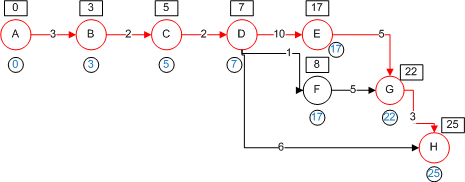
\includegraphics[width=130mm]{img/computation7.png}}}
\label{pic:plan7}
\caption{final project plan - critical path}
\end{figure}







\subsubsection{Checklist for Writing own CPM Spreadsheet / Software}
As a sumarry and when writing an own CPM Spreadsheet / Software, may it be in a Spreadsheet-Caclulation program like Microsoft Excel or even designing an own software the following rules/formulas must be defined:
\begin{itemize}
	\item The ES of the first activity is zero.
	\item The EF of any activity is $ES + D$.
	\item The ES of any activity is the latest of the EFs of all predecessors of that activity.
	\item The LF of the last activity in the project is equal to the EF of this activity. ($LF_{last} = EF_{last}$)
	\item The LS of any activity is $LF - D$
	\item The LF of any other activity except the last one is the earliest of all the LSs of all successors activities.
	\item The TF of any acitivity is equal to $LS - ES$ and also equal to $LF - EF$.
\end{itemize}
When following this rules a basic CPM-Algorithm can be implemented and the Project-Finish Date can be calculated after inputting a specific start date.













\section{Enhancements to the Basic System}
This section describes the most important enhancements of the basic CPM-System that have developed over time, and are found in the most recent software-CPM-programs. Some of these enhancements won't work with the basic formulas estabilished in \ref{formulas} but still keep the basic functionality in tact, others can be seen as just an extension of the basic system.

This list is in no way complete, since different programs implement different algorithms.

\subsection{Negative float}
When allowing a negative float in a CPM-System, one of the basic rules in the system "finish-to-start" is broken. This contraint is also called \textit{Finish not Later than (FNLT)}, which as seen by simple mathematics, if this FNLT-constraint is earlier than the standard LF, the Total Float will be a negative number.

With this FNLT constraint introduced there may arise some question to what is a critical activity now. For example if one activity has TF of minus two, does an activity with total float zero, which, by classic definition is a critical activity, still counts as critical? Furthermore, if the FNLT constraint is set to a later time then the calculated finish time, which value is used in further calculations? The answer to this last question depends on the program used, since there is no standard definition of this behaviour.

There also exists a SNLT (start not later than) contraint, which has the same problems as FNLT and should be used with caution as well.

\subsection{Actual Start and Finish Dates}

Another important Enhancement of the Standard CPM system is the ability to manually set start and finish dates. While it may be very convenient to just assign any single activity a specific value, this can lead to confusion depending on the exact algorithm used.

A typical problem is the "work out-of-sequence" with an activity started prior to completion of their predecessor activity.
There are many different ways in which software systems resolve this issue, among them:
\begin{itemize}
	\item Don't accept Inputs that may lead to this problem
	\item Write warning and generate output as good as possible
\end{itemize}

\subsection{User Defined Codes \& Resources}

Sometimes it is very helpful for an end-user to add additional informations or resources to an activity, for example a supervising person responsible for this activity. While this is helpful as additional Information, it should not be used to alter the network diagram in any way, or even assume that adding additional information is a replacement for other systems like any resource-managment-system. It can work in the small scale, but CPM is not made for managing to much additional information without compromising its original purpose.
An extra cost-field may be useful in determining if money can be saved by looking at the non-critical activities and evaluating if more time can lead to less cost, but cannot replace a cost-managment-system. 
\subsection{Calendars}

In the real word it is often the case that work can only be performed on work days (for example monday till friday) and even on these days only a specific amout of work-hours is possible. If activities are schedules in hours, this using calendars is very important concept.

On the other hand there are quite a few problems which need answering when using calendars:
\begin{itemize}
	\item \textbf{Float problem:} The TF depends on start and finish-date of an activity, but how is this calculated with weekend (non working days) in mind? For example if an activities ES is dated 1.1 and its LS 8.1, according to the formula $TF = LS - ES $ TF is 7 days. When considering a 5 day work calendar, the TF should only be 5 dys, since at least 1 weekend is in between. 
	\item Multi-calendar Problem: When working with multiple calendars at the same time, it may occur that an activity has 2 calendars assigned to it. For example an activity needs 2 limited Resources (see 
	
\end{itemize}




\section{Advantages and disadvantages}
Vor- und Nachteile (eventuell mit Alterntiven) (5 Seiten) - Thomas

\section{CPM in the field}
der Praxis: Programme (5 Seiten) - Clemens

%\section{Conclusion}
%(1 Seite)

\section{Sources}
\bibliography{sources}
\bibliographystyle{alpha}

\end{document}
